
PWM (Pulse Width Modulation) é um modulação baseada na conversão linear de um valor em escala de tensão para outro em escala de \emph{Duty Cicle} aplicado a uma onda quadrada de amplitude qualquer. Este tipo de modulação é utilizada em diversas aplicações eletrônicas. 

\section{Modos de Funcionamento}

Para criar uma modulação PWM é necessário criar uma onda periódica linear e variante no tempo, que se consiga comparar com o sinal que se deseja converter em PWM. Logo o tipo de onda necessária neste modulação é a onda triangular ou a onda dente de serra. Para melhor compreensão a onda triangular ou dente de serra será denominada aqui de onda portadora, e o sinal ao qual se deseja converter em PWM será denominado sinal modulante.
  
Para a implementação digital deste método pode ser feito através uma comparação direta entre os módulos dos dois sinais. Quando o modulo do sinal modulante for maior do que o  módulo da portadora  o sinal modulado vai para nível alto. Porém quando o módulo do sinal modulante for menor do que o módulo da portadora o sinal  modulado vai para zero. A grande diferença da implementação digital é que o sinal da portadora é gerado internamente através de um contador, que pode trabalhar no modo de contagem \emph{Down}, \emph{Up} ou \emph{UpDown}.

Quando o sinal da portadora é gerado através de um contador \emph{Down} ou \emph{Up}  a frequência do sinal modulado será igual a frequência do contador dividido pelo numero máximo de contagens. Já quando o sinal da portadora é gerador por um contador\emph{UpDown} a frequência do sinal modulado será igual a frequência do contador dividido por duas vezes o numero máximo de contagens. Sendo que o numero máximo de contagens deve ser maior ou igual ao modulo do sinal modulante. A Figura \ref{fig:Down} e a Figura \ref{fig:UpDown} apresentam melhor o modo como a geração de PWM é realizada digitalmente.  

\begin{figure}[H]
	\centering
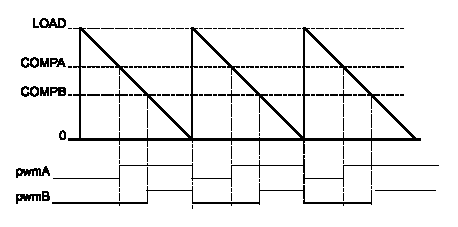
\includegraphics[width=0.8\textwidth] {figuras/Down.eps}
	\caption{PWM modo Down \cite{DATASHEET_TIVA}}
	\label{fig:Down}
\end{figure}

\begin{figure}[H]
	\centering
	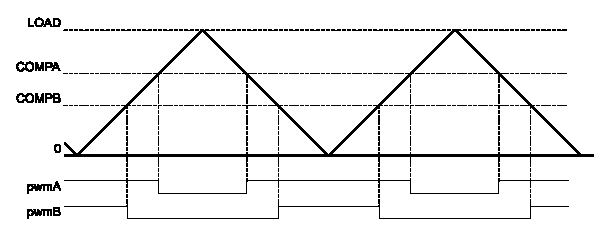
\includegraphics[width=0.8\textwidth] {figuras/UpDown.eps}
	\caption{PWM modo Down \cite{DATASHEET_TIVA}}
	\label{fig:UpDown}
\end{figure}

Tanto na Figura \ref{fig:Down} quanto na Figura \ref{fig:UpDown} os valores de \emph{LOAD}, \emph{COMPA}, \emph{COMPB}, \emph{pwmA} e \emph{pwmB} são referentes aos registradores presente do Tiva - TM4C1294NCPD, responsáveis pela modulação PWM. Tais registradores serão melhor abordados na próxima seção.  

\section{PWM do TM4C1294NCPDT}

O Tiva - TM4C1294NCPD possui um módulo PWM com quatro blocos geradores e seus respectivos blocos de controle, disponibilizando oito saídas PWM.  Através dos blocos de controle é possível escolher qual a polaridade de cada sinal PWM, e o seu respectivo pino. Cada bloco gerador produz 2 sinais PWM com a mesma frequência, porém ambos podem ter \emph{Duty Cicle} independentes ou \emph{Duty Cicle} complementares, com uma intervalo de \emph{Dead Band}. 

Como a maioria das aplicações com PWM é destinada ao chaveamento, o Tiva - TM4C1294NCPD possui não só uma configuração de geração PWM complementar com \emph{Dead Band}, recurso essencial para acionamento de pontes H, como também possui 4 pinos de entrada para um sistema de controle de falha, um para cada gerador PWM.

Para gerar a onda portadora o Tiva possui um contador de 16 bits capaz de realizar contagens no modo \emph{Down} e \emph{UpDown}, sendo possível atualizar o valor da contagem máxima (\emph{LOAD}). Cada um dos geradores PWM possuem ainda dois comparadores distintos (\emph{COMPA} e \emph{COMPB}), responsáveis por gerar os sinais PWM e que podem ser usados para gerar interrupções. 

Quando um comparador está configurado para provocar interrupções esta ocorre toda vez que o valor do comparador selecionado for maior do que o valor de \emph{LOAD}.  A Figura \ref{fig:PWMCountDownMode} demonstra o modo como as os sinais de interrupção são provocados pelos comparadores no modo \emph{Down}, e a Figura \ref{fig:PWMCountUpDownMode} demonstra o mesmo no modo \emph{UpDown}.

\begin{figure}[H]
	\centering
	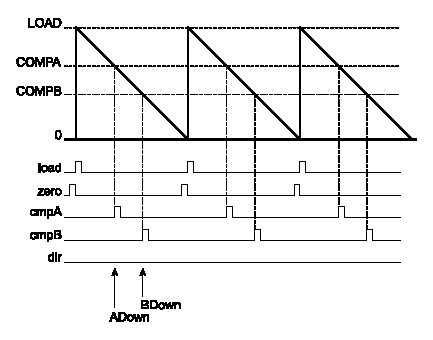
\includegraphics[width=0.8\textwidth] {figuras/PWMCountDownMode.eps}
	\caption{PWM modo Down \cite{DATASHEET_TIVA}}
	\label{fig:PWMCountDownMode}
\end{figure}

\begin{figure}[H]
	\centering
	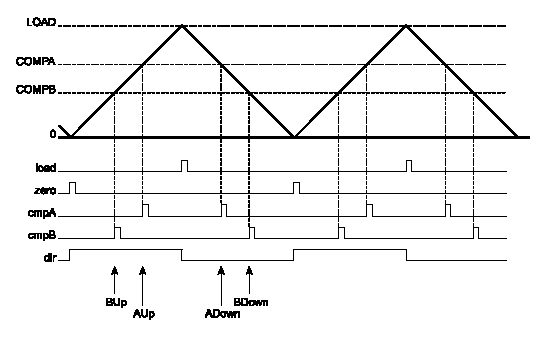
\includegraphics[width=0.8\textwidth] {figuras/PWMCountUpDownMode.eps}
	\caption{PWM modo Down \cite{DATASHEET_TIVA}}
	\label{fig:PWMCountUpDownMode}
\end{figure}

A tabela \ref{tab:CanaisPWM} apresenta os 8 pinos do módulo PWM, sendo estes pinos de saída dos sinais de PWM.  

\begin{center}
	\begin{longtable}{|c|c|c|c|c|}
		\rowcolor[HTML]{000000}
		{\color[HTML]{FFFFFF} Pino} & {\color[HTML]{FFFFFF} $n^{o}$} & {\color[HTML]{FFFFFF} Mux/Função} & {\color[HTML]{FFFFFF} Tipo} & {\color[HTML]{FFFFFF} Descrição}            \\
		M0PWM0    & 42  & PF0 (6) & O & Saída PWM 0\\
		M0PWM1    & 43  & PF1 (6) & O & Saída PWM 1\\
		M0PWM2    & 44  & PF2 (6) & O & Saída PWM 2\\
		M0PWM3    & 45  & PF3 (6) & O & Saída PWM 3\\
		M0PWM4    & 49  & PG0 (6) & O & Saída PWM 4\\
		M0PWM5    & 50  & PG1 (6) & O & Saída PWM 5\\
		M0PWM6    & 63  & PK4 (6) & O & Saída PWM 6\\
		M0PWM7    & 62  & PK5 (6) & O & Saída PWM 7\\
		\hline
		\caption{Canais PWM - Tiva TM4C1294NCPDT \cite{DATASHEET_TIVA} }
		\label{tab:CanaisPWM}
	\end{longtable}
\end{center}

\section{PWM do TM4C1294NCPDT}

\section{Exemplo}
